%picture of panel antenna setup, including amplifier
This section applies the knowledge gained in the previous section to detect the presence of unknown code at a distance of 3 meters. We used the antenna with the highest gain (the 18 dBi panel antenna) and the same replace benchmark with the same training and evaluation inputs as used in Chapter~\ref{zop}. As we determined in Section~\ref{malware-dist-static}, this training set has poor coverage of some portions of this benchmark. While it is expected that better input generation will improve ZOP's performance, but generating inputs with thorough coverage of large programs is challenging. Therefore we will continue to use this training input set because ZOP needs to be robust against training inputs that do not provide perfect coverage. 

In this measurement we will evaluate whether ZOP can predict when unknown code is present in a given program execution. For this purpose, we will not use any of the training waveforms which describe a particular function (the \texttt{putsub} function) in the replace benchmark. Therefore, when ZOP encounters calls to this function, it will attempt to match the unknown waveform to only to training waveforms for the valid known code paths, but not to the \texttt{putsub} function. These waveforms will not match well against the unknown waveform because the unknown waveforms were recorded during different program activity (i.e. the \texttt{putsub} function). In other words, the waveform matching is expected to be good when ZOP encounters known code (i.e. code for which it has training examples), and poor when ZOP encounters unknown code (i.e. code with no training examples). Therefore, if we look at the matching between to-be-predicted waveform and the training example waveforms ZOP picks as the best matches to the to-be-predicted waveform during a period of time where code is executing for which we have no training examples, we would expect that the matching will be very poor (i.e. have a low correlation). 

We can use the fact that the best matching training examples will have low correlation to unknown code to determine whether a given execution contains unknown code. To do this, for a given execution, for each predicted marker in the predicted marker sequence, we look at the correlation between the highest correlated training example waveform (which was used to selected this marker in the final prediction) and the to-be-predicted waveform. This gives us a list of correlations between the highest correlated training waveform and the to-be-predicted waveform for short sections of the waveform recorded for the entire duration of the program's execution. Then, for each executed input, we find the minimum correlation in this list, and assign that value to that executed input. This gives us a score that is likely to be lower when unknown code is present for a particular executed input.

We ran ZOP for the same set of 400 evaluation inputs described in Chapter~\ref{zop} with the same training input set, removing only the training examples which correspond to the unknown code. Out of 400 evaluation inputs, 69 inputs contained at least one call to the \texttt{putsub} function. Figure~\ref{malware_detect} shows histograms of the results. The x-axis shows the minimum correlation of each input as described above and the y-axis shows the number of evaluation inputs which had that minimum correlation. The red distribution shows the inputs that executed some unknown code and the blue distribution shows the inputs that contained no unknown code. 

\begin{figure}[hbt]
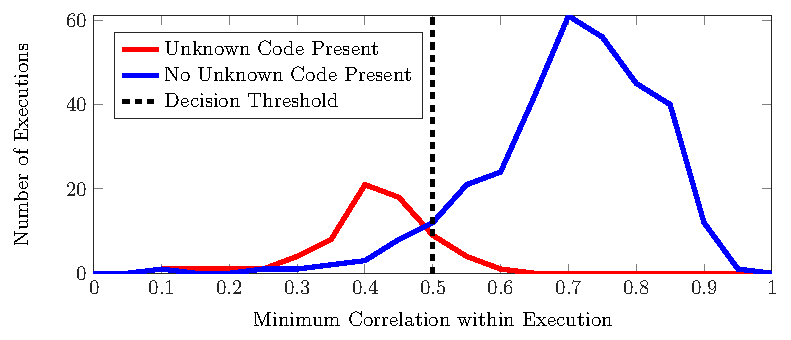
\includegraphics[width=5in]{malware_detect}
\caption{Histograms of the number of executions with a given minimum correlation for the executions with unknown code (red) and containing only known code (blue).}
\label{malware_detect}
\end{figure}

In order to determine a final performance metric (e.g. the number of false positives and negatives) a decision threshold must be chosen. To predict whether unknown code was executed for a given input we look at the minimum correlation over that input. If this correlation is below the decision threshold, we predict unknown code is present and if the correlation is above the threshold, we predict unknown code is not present. While there is some overlap between the distributions, they are separated enough that a decision threshold can be chosen to accurately determine whether a given input contains unknown code. For example, if we pick a decision threshold of 0.5 (as shown by the dotted black line in Figure~\ref{malware_detect}), we will correctly classify 92\% of the executed inputs with 6\% false positives (inputs that don't actually execute unknown code but are predicted to execute unknown code) and 2\% false negatives (inputs with unknown code predicted to not contain unknown code). This prediction threshold gives the optimal accuracy for this particular measurement but a user may wish to set a different decision threshold (e.g. to reduce the number of false positives). Furthermore, the optimal decision threshold will depend on the signal quality for a particular measurement setup, since lower signal quality will result in lower correlation overall.


